\subsection{Datasets} \label{subsec:datasets}

We evaluate on three datasets: a multi-dimensional synthetic set, a 2D adversarial synthetic set, and the EUC\_2D subset of TSPLIB95. The synthetic sets are held-out test splits from our generation pipeline (Appendix~\ref{app:training}); TSPLIB95 is real-world.

\subsubsection{Multi-dimensional synthetic ($d = 2$--$100$)}
16{,}907 held-out instances with $n \in [5, 1000]$ and $d \in \{2, 3, \ldots, 50, 100\}$, sampled by stratified dimension--size--grid buckets across 16 distribution types per dimension (uniform, Gaussian, clustered, anisotropic, structured). Stratification enforces zero overlap with the training split. $d = 100$ is outside the training range and serves as the extrapolation test.

\subsubsection{2D adversarial synthetic}
2{,}580 instances, $d = 2$, $n \in [5, 1000]$, coordinate grid side-length $G \in [1000, 10000]$. Five distribution classes (Table~\ref{tab:dataset_counts}) each target a classical estimator assumption. The \textit{Line Noise} class contains 210 near-linear manifolds of the form $y = mx + b + \epsilon$ with small $\epsilon$. As $\epsilon \to 0$ the convex hull area approaches zero and the bounding-box area stays finite, so any estimator of the form $\hat L \propto \sqrt{A}$ collapses to zero or overestimates wildly, depending on which enclosure is chosen. We include these deliberately to probe the hull/box dilemma in BHH, Cavdar, and Chien.

\begin{table}[!ht]
\centering
\caption{2D benchmark dataset composition (2{,}580 instances total).}
\label{tab:dataset_counts}
\resizebox{\textwidth}{!}{%
\begin{tabular}{@{}llcp{6cm}@{}}
\toprule
\textbf{Class} & \textbf{Generators} & \textbf{Count} & \textbf{Stress target} \\ \midrule
Isotropic Noise & Uniform, Normal, Triangular, Truncated Exp. & 840 & Control: $A_{\text{hull}} \approx A_{\text{box}}$. \\
Biased / Skewed & Squeezed, Uni-Tri, Tri-Squeezed, Correlated & 840 & Aspect-ratio distortion: $\sigma_x \neq \sigma_y$. \\
Geometric Struct. & Grid, Boundary (hollow), X-Central & 630 & Lattice regularity, hollow voids. \\
Clustered & $k$-Means ($k \in [5, 20]$) & 60 & Bimodal edge-weight distribution. \\
Line Noise & Linear manifold + $\epsilon$ & 210 & Hull/box divergence as data collapses to 1D. \\ \midrule
\textbf{Total} & & \textbf{2{,}580} & \\
\bottomrule
\end{tabular}%
}
\end{table}

\subsubsection{TSPLIB95 EUC\_2D common subset}
78 EUC\_2D instances with $n$ from 14 to 85{,}900 \citep{reinelt1991tsplib}. This is the intersection where every benchmark model is directly applicable: all five classical baselines require 2D Euclidean coordinates, and the MST Ratio baseline needs only a distance matrix. The remaining 33 TSPLIB95 instances (CEIL\_2D, ATT pseudo-Euclidean, GEO great-circle, EXPLICIT distance-matrix) are not natively Euclidean and are evaluated in Section~\ref{sec:application} via MDS embedding, which only GART 3.0 supports. For large instances where the dense $n \times n$ distance matrix would exceed memory, we replace it with a Delaunay-based MST construction \citep{delaunay1934} that uses only $O(n)$ edges.

\subsection{Results} \label{subsec:results}

Every table below reports the same seven quantities per model: instance count $N$, MAPE, SDPE, median $|\%\text{error}|$, $R^2$ on tour cost, $R^2_\alpha$ on the MST--TSP ratio (only for models that predict $\alpha$ directly), and mean total prediction time in milliseconds (feature extraction + MST + inference).

\subsubsection{Multi-dimensional benchmark} \label{subsec:results_nd}

We present the 16{,}907-instance multi-dimensional benchmark in two orthogonal slices: by instance size (Table~\ref{tab:nd_by_size}) and by dimension (Table~\ref{tab:nd_by_dim}). Both tables summarize the same underlying data; we show both for editorial review.

\begin{table}[!ht]
\centering
\caption{ND benchmark sliced by instance size. Same 16{,}907 instances as Table~\ref{tab:nd_by_dim}.}
\label{tab:nd_by_size}
\resizebox{\textwidth}{!}{%
\footnotesize
\begin{tabular}{@{}ll rrrrrrr@{}}
\toprule
$n$ bucket & Model & $N$ & MAPE (\%) & SDPE (\%) & Median (\%) & $R^2$ & $R^2_\alpha$ & Time (ms) \\
\midrule
\multirow{3}{*}{$[5,10]$}     & GART 3.0  & 4{,}227 & \textbf{1.36} & \textbf{1.90} & 0.99 & 0.9999 & 0.943 & 108.2 \\
                              & MST Ratio & 4{,}227 & 18.89 & 5.44 & 17.89 & 0.966 & $-4.631$ & 6.7 \\
                              & Hilbert   & 4{,}227 & 8.11 & 7.45 & 5.75 & 0.995 & --- & 15.6 \\ \midrule
\multirow{3}{*}{$[11,50]$}    & GART 3.0  & 2{,}816 & \textbf{0.88} & \textbf{1.17} & 0.73 & 0.9999 & 0.928 & 109.6 \\
                              & MST Ratio & 2{,}816 & 7.45 & 2.89 & 6.94 & 0.997 & $-2.077$ & 17.2 \\
                              & Hilbert   & 2{,}816 & 19.59 & 12.35 & 15.60 & 0.981 & --- & 37.8 \\ \midrule
\multirow{3}{*}{$[51,100]$}   & GART 3.0  & 3{,}522 & \textbf{0.66} & \textbf{0.79} & 0.58 & 0.9999 & 0.950 & 110.3 \\
                              & MST Ratio & 3{,}522 & 5.33 & 2.13 & 4.80 & 0.998 & $-1.371$ & 28.4 \\
                              & Hilbert   & 3{,}522 & 24.38 & 14.10 & 20.18 & 0.973 & --- & 73.3 \\ \midrule
\multirow{3}{*}{$[101,200]$}  & GART 3.0  & 703 & \textbf{0.55} & \textbf{0.63} & 0.47 & 0.9999 & 0.958 & 110.8 \\
                              & MST Ratio & 703 & 4.44 & 1.74 & 4.12 & 0.999 & $-1.103$ & 47.5 \\
                              & Hilbert   & 703 & 27.03 & 13.61 & 23.40 & 0.965 & --- & 155.4 \\ \midrule
\multirow{3}{*}{$[201,500]$}  & GART 3.0  & 2{,}115 & \textbf{0.50} & \textbf{0.56} & 0.39 & 0.9999 & 0.956 & 107.1 \\
                              & MST Ratio & 2{,}115 & 4.06 & 1.51 & 3.80 & 0.999 & $-1.097$ & 75.9 \\
                              & Hilbert   & 2{,}115 & 28.26 & 12.75 & 26.22 & 0.960 & --- & 238.6 \\ \midrule
\multirow{3}{*}{$[501,1000]$} & GART 3.0  & 3{,}524 & \textbf{0.49} & \textbf{0.55} & 0.31 & 0.9998 & 0.949 & 108.5 \\
                              & MST Ratio & 3{,}524 & 3.82 & 1.32 & 3.63 & 0.999 & $-1.134$ & 212.8 \\
                              & Hilbert   & 3{,}524 & 29.97 & 12.77 & 28.71 & 0.953 & --- & 1027.9 \\ \midrule
\multirow{3}{*}{\textbf{ALL}} & \textbf{GART 3.0}  & \textbf{16{,}907} & \textbf{0.81} & \textbf{1.17} & \textbf{0.63} & \textbf{0.9999} & \textbf{0.978} & \textbf{330.0} \\
                              & MST Ratio & 16{,}907 & 8.56 & 6.89 & 5.61 & 0.999 & $-0.834$ & 132.5 \\
                              & Hilbert   & 16{,}907 & 21.28 & 14.55 & 16.22 & 0.962 & --- & 552.1 \\
\bottomrule
\end{tabular}%
}
\end{table}

\begin{table}[!ht]
\centering
\caption{ND benchmark sliced by dimension. Same 16{,}907 instances as Table~\ref{tab:nd_by_size}. $d = 100$ is outside the training range (extrapolation).}
\label{tab:nd_by_dim}
\resizebox{\textwidth}{!}{%
\footnotesize
\begin{tabular}{@{}ll rrrrrrr@{}}
\toprule
$d$ bucket & Model & $N$ & MAPE (\%) & SDPE (\%) & Median (\%) & $R^2$ & $R^2_\alpha$ & Time (ms) \\
\midrule
\multirow{3}{*}{$d=2$}           & GART 3.0  & 647 & \textbf{1.82} & \textbf{2.75} & 0.99 & 0.9999 & 0.955 & 106.1 \\
                                 & MST Ratio & 647 & 13.19 & 10.70 & 8.95 & 0.995 & $-0.983$ & 49.0 \\
                                 & Hilbert   & 647 & 30.36 & 16.41 & 35.31 & 0.805 & --- & 41.4 \\ \midrule
\multirow{3}{*}{$d=3$--$5$}      & GART 3.0  & 1{,}941 & \textbf{1.16} & \textbf{1.83} & 0.64 & 1.000 & 0.962 & 108.2 \\
                                 & MST Ratio & 1{,}941 & 11.72 & 8.07 & 8.02 & 0.996 & $-1.376$ & 48.8 \\
                                 & Hilbert   & 1{,}941 & 35.53 & 15.82 & 39.96 & 0.737 & --- & 52.3 \\ \midrule
\multirow{3}{*}{$d=6$--$10$}     & GART 3.0  & 3{,}240 & \textbf{0.83} & \textbf{1.28} & 0.48 & 1.000 & 0.971 & 108.9 \\
                                 & MST Ratio & 3{,}240 & 10.27 & 6.64 & 7.19 & 0.997 & $-1.674$ & 51.4 \\
                                 & Hilbert   & 3{,}240 & 32.78 & 14.34 & 36.20 & 0.789 & --- & 78.4 \\ \midrule
\multirow{3}{*}{$d=15$--$25$}    & GART 3.0  & 1{,}944 & \textbf{0.54} & \textbf{0.84} & 0.31 & 1.000 & 0.984 & 110.0 \\
                                 & MST Ratio & 1{,}944 & 8.72 & 6.02 & 5.70 & 0.998 & $-1.570$ & 56.8 \\
                                 & Hilbert   & 1{,}944 & 24.73 & 11.81 & 26.33 & 0.846 & --- & 147.7 \\ \midrule
\multirow{3}{*}{$d=30$--$50$}    & GART 3.0  & 3{,}236 & \textbf{0.36} & \textbf{0.58} & 0.20 & 1.000 & 0.992 & 109.0 \\
                                 & MST Ratio & 3{,}236 & 7.63 & 5.90 & 4.60 & 0.999 & $-1.301$ & 63.7 \\
                                 & Hilbert   & 3{,}236 & 17.14 & 7.98 & 18.13 & 0.924 & --- & 247.2 \\ \midrule
\multirow{3}{*}{$d=100^{*}$}     & GART 3.0  & 5{,}899 & \textbf{0.90} & \textbf{0.50} & 0.89 & 1.000 & 0.980 & 109.0 \\
                                 & MST Ratio & 5{,}899 & 6.54 & 5.93 & 3.43 & 0.999 & $-0.995$ & 86.6 \\
                                 & Hilbert   & 5{,}899 & 10.40 & 4.60 & 11.08 & 0.971 & --- & 542.0 \\ \midrule
\multirow{3}{*}{\textbf{ALL}}    & \textbf{GART 3.0}  & \textbf{16{,}907} & \textbf{0.81} & \textbf{1.17} & \textbf{0.63} & \textbf{0.9999} & \textbf{0.978} & \textbf{330.0} \\
                                 & MST Ratio & 16{,}907 & 8.56 & 6.89 & 5.61 & 0.999 & $-0.834$ & 132.5 \\
                                 & Hilbert   & 16{,}907 & 21.28 & 14.55 & 16.22 & 0.962 & --- & 552.1 \\
\bottomrule
\multicolumn{9}{l}{\footnotesize $^{*}$ $d = 100$ is outside the training range; included to test extrapolation.}
\end{tabular}%
}
\end{table}

\begin{figure}[!ht]
\centering
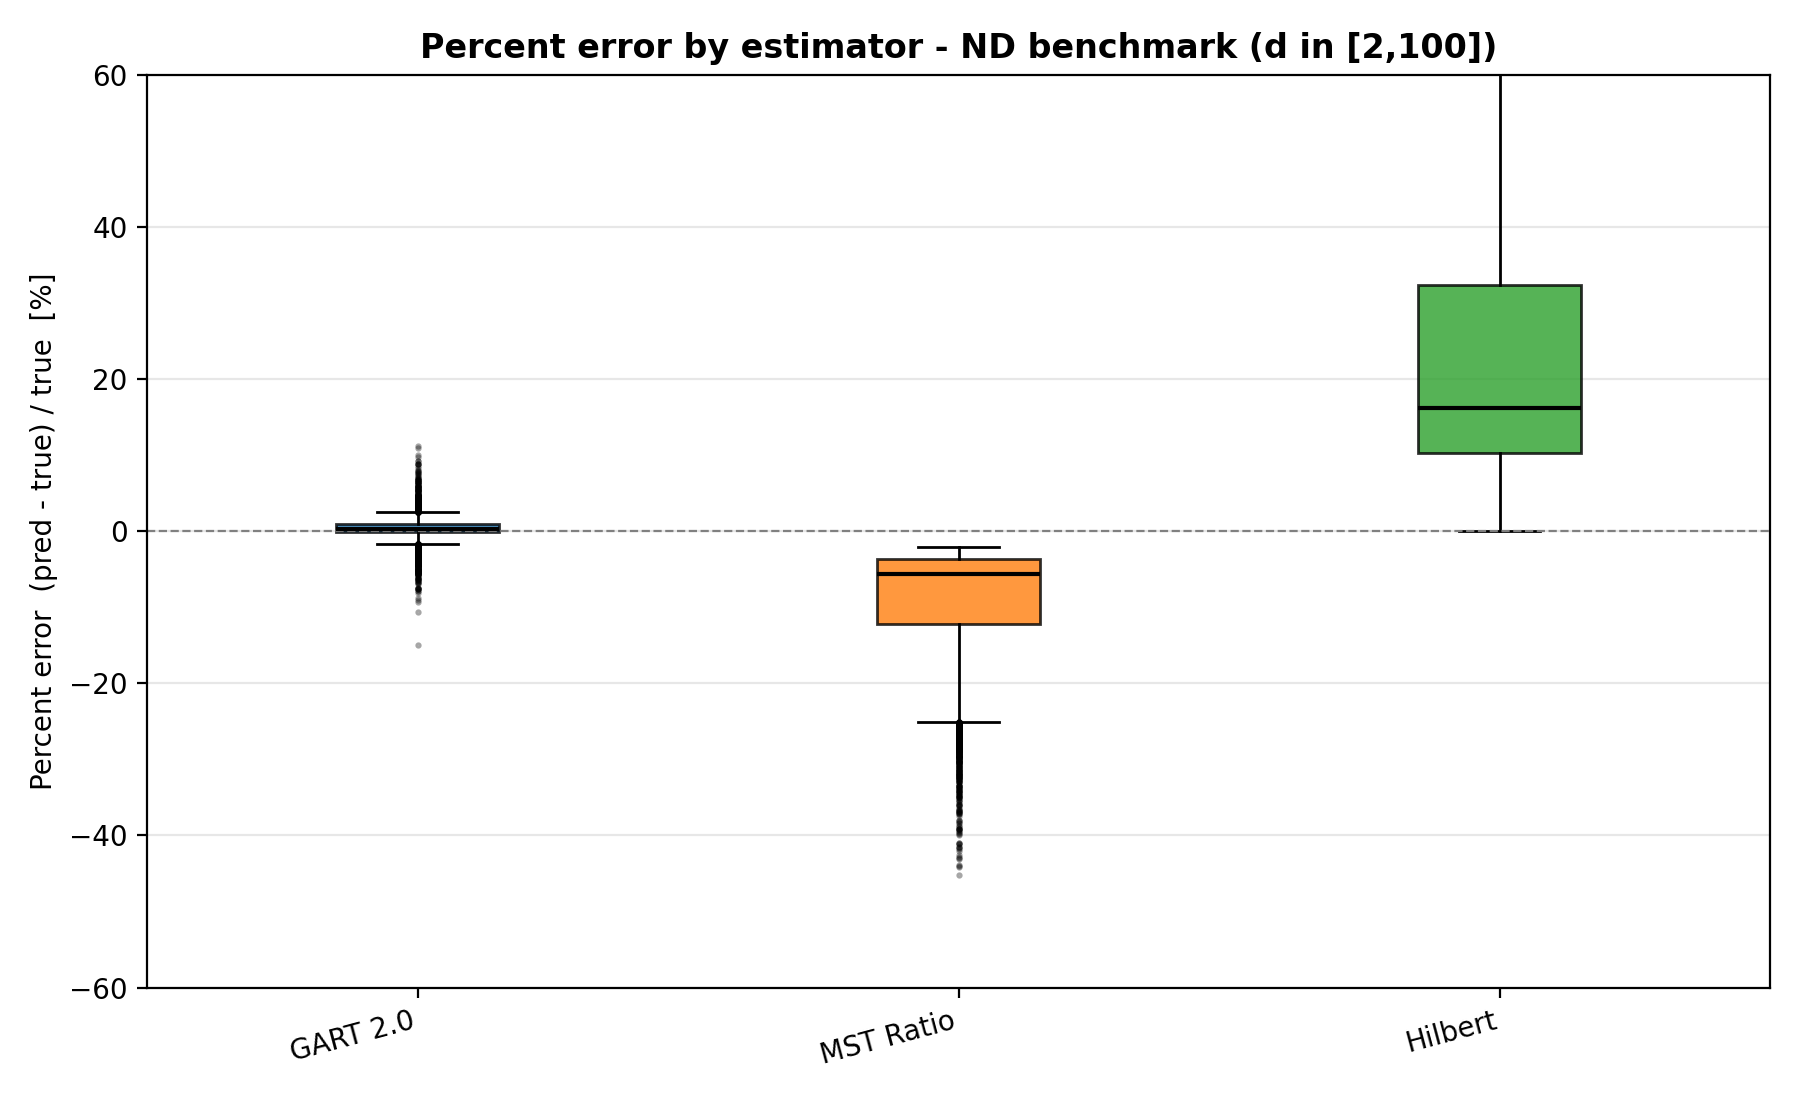
\includegraphics[width=0.75\textwidth]{boxplot_nd_errors.png}
\caption{Percent-error distribution per model on the ND benchmark (16{,}907 instances).}
\label{fig:boxplot_nd}
\end{figure}

GART 3.0 reaches 0.81\% MAPE and 1.17\% SDPE overall, against 8.56\% / 6.89\% for MST Ratio and 21.28\% / 14.55\% for Hilbert. Precision tightens monotonically as $n$ grows (SDPE drops from 1.90\% at $n \le 10$ to 0.55\% at $n \ge 500$) and also as $d$ grows (2.75\% at $d = 2$ down to 0.50\% at $d = 100$), consistent with the theoretical convergence $\alpha \to 1$ in high dimensions \citep{percus1996}. MST Ratio's SDPE is nearly flat because its fixed constant cannot adapt to instance structure. Hilbert degrades with $n$ because space-filling locality breaks on non-uniform distributions.

\subsubsection{2D adversarial benchmark} \label{subsec:results_2d}

Table~\ref{tab:2d_by_size} disaggregates the 2{,}580-instance 2D benchmark by instance size.

\begin{table}[!ht]
\centering
\caption{2D adversarial benchmark by instance size (2{,}580 instances). $R^2_\alpha$ is derivable only for models that predict $\alpha$ directly.}
\label{tab:2d_by_size}
\resizebox{\textwidth}{!}{%
\footnotesize
\begin{tabular}{@{}ll rrrrrrr@{}}
\toprule
$n$ bucket & Model & $N$ & MAPE (\%) & SDPE (\%) & Median (\%) & $R^2$ & $R^2_\alpha$ & Time (ms) \\
\midrule
\multirow{6}{*}{$[5,10]$}    & GART 3.0  & 360 & \textbf{4.53} & \textbf{5.53} & 3.80 & 0.993 & 0.861 & 61.5 \\
                             & MST Ratio & 360 & 28.95 & 9.99 & 29.17 & 0.785 & $-0.766$ & 4.9 \\
                             & Cavdar    & 360 & 17.37 & 14.25 & 13.18 & 0.904 & --- & 3.3 \\
                             & BHH       & 360 & 59.32 & 9.74 & 57.70 & 0.203 & --- & 3.9 \\
                             & Chien     & 360 & 25.81 & 7.23 & 26.24 & 0.842 & --- & 0.6 \\
                             & Hilbert   & 360 & 8.35 & 8.84 & 5.79 & 0.965 & --- & 1.8 \\ \midrule
\multirow{6}{*}{$[11,50]$}   & GART 3.0  & 480 & \textbf{4.18} & \textbf{5.87} & 2.77 & 0.994 & 0.861 & 54.9 \\
                             & MST Ratio & 480 & 15.16 & 9.66 & 13.63 & 0.949 & $-0.766$ & 7.6 \\
                             & Cavdar    & 480 & 12.73 & 16.28 & 8.45 & 0.943 & --- & 4.4 \\
                             & BHH       & 480 & 28.38 & 9.28 & 27.64 & 0.817 & --- & 4.5 \\
                             & Chien     & 480 & 19.64 & 18.68 & 17.88 & 0.888 & --- & 0.6 \\
                             & Hilbert   & 480 & 27.18 & 10.37 & 26.95 & 0.804 & --- & 1.5 \\ \midrule
\multirow{6}{*}{$[51,100]$}  & GART 3.0  & 630 & \textbf{3.57} & \textbf{5.53} & 2.05 & 0.995 & 0.861 & 71.3 \\
                             & MST Ratio & 630 & 11.45 & 8.59 & 9.34 & 0.975 & $-0.766$ & 14.7 \\
                             & Cavdar    & 630 & 19.07 & 29.40 & 7.45 & 0.897 & --- & 4.3 \\
                             & BHH       & 630 & 16.22 & 13.08 & 14.98 & 0.912 & --- & 5.5 \\
                             & Chien     & 630 & 23.38 & 30.74 & 16.69 & 0.853 & --- & 0.3 \\
                             & Hilbert   & 630 & 34.23 & 9.82 & 34.08 & 0.734 & --- & 1.9 \\ \midrule
\multirow{6}{*}{$[101,200]$} & GART 3.0  & 120 & \textbf{2.86} & \textbf{5.03} & 1.30 & 0.996 & 0.861 & 87.3 \\
                             & MST Ratio & 120 & 8.31 & 7.06 & 6.72 & 0.989 & $-0.766$ & 16.3 \\
                             & Cavdar    & 120 & 18.70 & 41.03 & 3.36 & 0.911 & --- & 3.9 \\
                             & BHH       & 120 & 11.82 & 20.23 & 6.85 & 0.946 & --- & 5.1 \\
                             & Chien     & 120 & 25.75 & 42.94 & 15.23 & 0.853 & --- & 0.2 \\
                             & Hilbert   & 120 & 36.61 & 10.48 & 36.48 & 0.717 & --- & 3.7 \\ \midrule
\multirow{6}{*}{$[201,500]$} & GART 3.0  & 380 & \textbf{2.48} & \textbf{4.22} & 1.14 & 0.997 & 0.861 & 61.6 \\
                             & MST Ratio & 380 & 7.19 & 6.04 & 5.94 & 0.992 & $-0.766$ & 41.5 \\
                             & Cavdar    & 380 & 26.11 & 55.60 & 3.21 & 0.867 & --- & 7.1 \\
                             & BHH       & 380 & 15.35 & 32.05 & 4.26 & 0.927 & --- & 4.9 \\
                             & Chien     & 380 & 30.90 & 56.03 & 14.49 & 0.823 & --- & 2.9 \\
                             & Hilbert   & 380 & 38.59 & 9.94 & 38.21 & 0.717 & --- & 19.5 \\ \midrule
\multirow{6}{*}{$[501,1000]$}& GART 3.0  & 610 & \textbf{1.92} & \textbf{3.16} & 0.95 & 0.997 & 0.861 & 73.6 \\
                             & MST Ratio & 610 & 5.71 & 4.54 & 5.00 & 0.994 & $-0.766$ & 118.4 \\
                             & Cavdar    & 610 & 23.93 & 58.54 & 3.39 & 0.872 & --- & 12.6 \\
                             & BHH       & 610 & 14.75 & 33.64 & 5.08 & 0.931 & --- & 8.0 \\
                             & Chien     & 610 & 29.90 & 59.34 & 14.07 & 0.823 & --- & 7.0 \\
                             & Hilbert   & 610 & 38.24 & 11.17 & 38.21 & 0.728 & --- & 46.9 \\ \midrule
\multirow{6}{*}{\textbf{ALL}}& \textbf{GART 3.0}  & \textbf{2{,}580} & \textbf{3.23} & \textbf{4.94} & \textbf{1.73} & \textbf{0.998} & \textbf{0.861} & \textbf{66.7} \\
                             & MST Ratio & 2{,}580 & 12.45 & 11.06 & 8.16 & 0.992 & $-0.766$ & 40.5 \\
                             & Cavdar    & 2{,}580 & 19.82 & 42.04 & 6.13 & 0.909 & --- & 6.6 \\
                             & BHH       & 2{,}580 & 23.82 & 32.05 & 15.55 & 0.943 & --- & 5.6 \\
                             & Chien     & 2{,}580 & 25.78 & 42.55 & 17.25 & 0.874 & --- & 2.4 \\
                             & Hilbert   & 2{,}580 & 31.01 & 14.24 & 34.99 & 0.801 & --- & 15.1 \\
\bottomrule
\end{tabular}%
}
\end{table}

\begin{figure}[!ht]
\centering
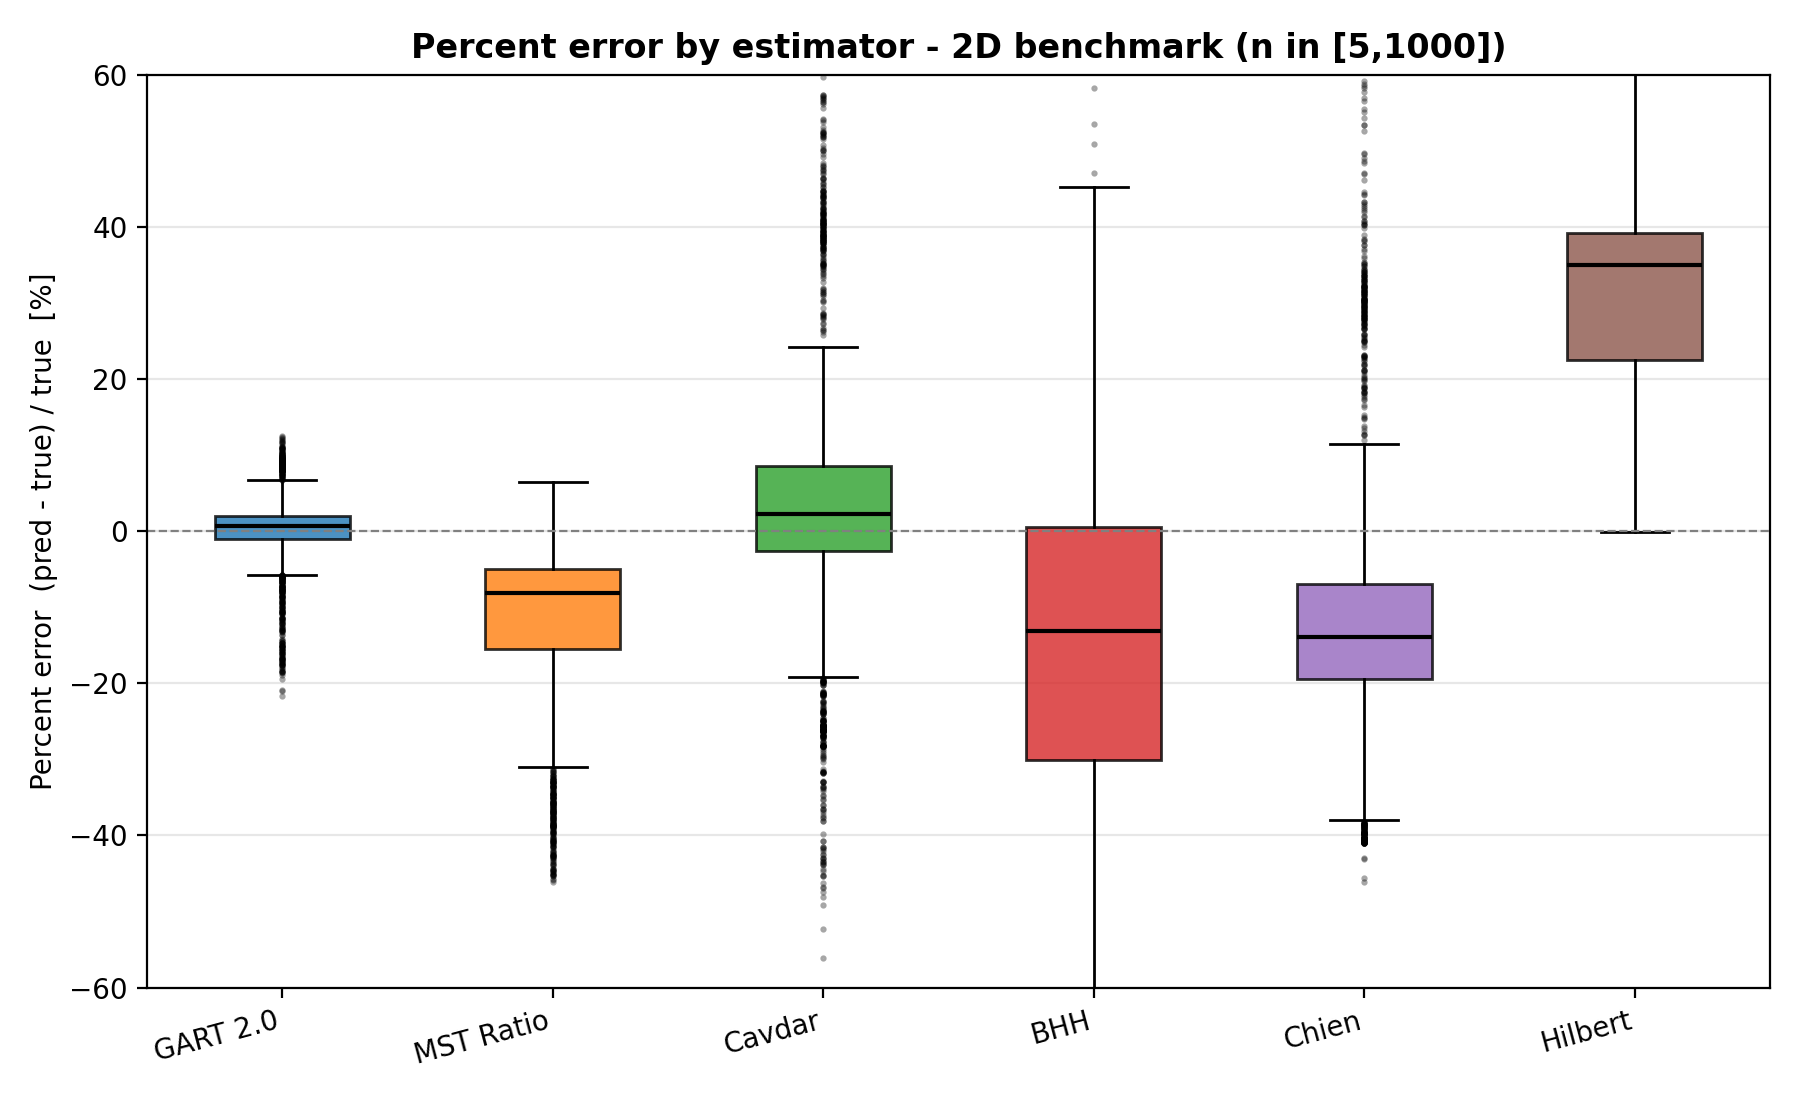
\includegraphics[width=0.75\textwidth]{boxplot_2d_errors.png}
\caption{Percent-error distribution per model on the 2D adversarial benchmark (2{,}580 instances).}
\label{fig:boxplot_2d}
\end{figure}

GART 3.0 leads at 3.23\% MAPE / 4.94\% SDPE overall. MST Ratio is second at 12.45\% / 11.06\%. Cavdar, BHH, and Chien all exceed 30\% SDPE because their enclosure-based formulas amplify variance on the Biased and Line Noise classes, where bounding-box and hull volumes diverge. Hilbert has intermediate MAPE (31\%) but relatively low SDPE (14\%): its errors are large but consistent --- a systematic space-filling bias. GART's SDPE $R^2_\alpha = 0.861$ is the only non-negative value among direct-$\alpha$ predictors, confirming that the model captures per-instance $\alpha$ variation beyond what a fixed ratio can.

\subsubsection{TSPLIB95 EUC\_2D benchmark} \label{subsec:results_tsplib}

Table~\ref{tab:tsplib_by_size} reports per-size-bucket results across all 78 EUC\_2D instances, with $n$ from 14 (\texttt{burma14}) to 85{,}900 (\texttt{pla85900}).

\begin{table}[!ht]
\centering
\caption{TSPLIB95 EUC\_2D benchmark by instance size (78 instances, $n \in [14, 85{,}900]$).}
\label{tab:tsplib_by_size}
\resizebox{\textwidth}{!}{%
\footnotesize
\begin{tabular}{@{}ll rrrrrrr@{}}
\toprule
$n$ bucket & Model & $N$ & MAPE (\%) & SDPE (\%) & Median (\%) & $R^2$ & $R^2_\alpha$ & Time (ms) \\
\midrule
\multirow{6}{*}{$n < 100$}        & GART 3.0  & 6 & \textbf{2.64} & \textbf{3.33} & 1.78 & 0.997 & 0.617 & 2.9 \\
                                  & MST Ratio & 6 & 8.02 & 4.96 & 7.72 & 0.978 & $-2.832$ & 7.0 \\
                                  & Cavdar    & 6 & 8.39 & 10.89 & 7.38 & 0.994 & --- & 3.1 \\
                                  & BHH       & 6 & 22.18 & 6.19 & 21.07 & 0.975 & --- & 3.2 \\
                                  & Chien     & 6 & 23.50 & 6.73 & 23.86 & 0.943 & --- & 1.1 \\
                                  & Hilbert   & 6 & 34.61 & 9.12 & 34.60 & 0.788 & --- & 1.4 \\ \midrule
\multirow{6}{*}{$[100, 500)$}     & GART 3.0  & 37 & \textbf{3.11} & \textbf{3.36} & 2.26 & 0.996 & 0.237 & 3.3 \\
                                  & MST Ratio & 37 & 6.31 & 4.37 & 5.18 & 0.983 & $-1.736$ & 29.6 \\
                                  & Cavdar    & 37 & 17.40 & 25.07 & 7.94 & 0.724 & --- & 8.3 \\
                                  & BHH       & 37 & 17.48 & 25.59 & 11.46 & 0.851 & --- & 8.9 \\
                                  & Chien     & 37 & 20.64 & 24.87 & 16.96 & 0.895 & --- & 2.4 \\
                                  & Hilbert   & 37 & 43.22 & 9.74 & 41.77 & 0.597 & --- & 4.1 \\ \midrule
\multirow{6}{*}{$[500, 1000]$}    & GART 3.0  & 6 & \textbf{2.86} & \textbf{3.84} & 1.85 & 0.992 & $-0.938$ & 3.3 \\
                                  & MST Ratio & 6 & 4.23 & 3.46 & 4.54 & 0.983 & $-1.722$ & 96.5 \\
                                  & Cavdar    & 6 & 21.94 & 41.85 & 7.30 & 0.241 & --- & 24.6 \\
                                  & BHH       & 6 & 30.87 & 58.98 & 10.25 & $-0.511$ & --- & 28.4 \\
                                  & Chien     & 6 & 33.66 & 53.33 & 21.67 & $-0.036$ & --- & 8.3 \\
                                  & Hilbert   & 6 & 46.36 & 3.15 & 46.97 & 0.069 & --- & 12.8 \\ \midrule
\multirow{6}{*}{$(1000, 5000]$}   & GART 3.0  & 22 & \textbf{4.34} & \textbf{3.86} & 2.62 & 0.996 & $-0.670$ & 12.3 \\
                                  & MST Ratio & 22 & 4.09 & 4.20 & 4.33 & 0.992 & $-0.387$ & 329.1 \\
                                  & Cavdar    & 22 & 36.58 & 53.95 & 19.63 & 0.789 & --- & 75.6 \\
                                  & BHH       & 22 & 38.61 & 55.71 & 22.59 & 0.797 & --- & 86.1 \\
                                  & Chien     & 22 & 31.56 & 49.47 & 16.63 & 0.912 & --- & 20.2 \\
                                  & Hilbert   & 22 & 49.59 & 14.69 & 48.07 & 0.174 & --- & 37.4 \\ \midrule
\multirow{6}{*}{$n > 5000$}       & GART 3.0  & 7 & \textbf{4.84} & \textbf{3.43} & 4.60 & 0.995 & --- & 149.1 \\
                                  & MST Ratio & 7 & 4.14 & 2.75 & 3.98 & 0.996 & --- & 858.8 \\
                                  & Cavdar    & 7 & 25.42 & 20.48 & 22.46 & 0.813 & --- & 230.3 \\
                                  & BHH       & 7 & 28.66 & 22.91 & 19.90 & 0.844 & --- & 269.8 \\
                                  & Chien     & 7 & 24.03 & 19.12 & 23.80 & 0.931 & --- & 48.2 \\
                                  & Hilbert   & 7 & 48.24 & 7.32 & 48.16 & 0.524 & --- & 171.0 \\ \midrule
\multirow{6}{*}{\textbf{ALL}}     & \textbf{GART 3.0}  & \textbf{78} & \textbf{3.44} & \textbf{3.52} & \textbf{2.37} & \textbf{1.000} & \textbf{0.163} & \textbf{36.7} \\
                                  & MST Ratio & 78 & 5.22 & 4.54 & 4.96 & 0.998 & $-1.006$ & 170.6 \\
                                  & Cavdar    & 78 & 22.95 & 36.30 & 11.44 & 0.833 & --- & 1.7 \\
                                  & BHH       & 78 & 25.16 & 40.75 & 13.41 & 0.880 & --- & 1.9 \\
                                  & Chien     & 78 & 24.05 & 35.83 & 16.84 & 0.934 & --- & 0.9 \\
                                  & Hilbert   & 78 & 45.20 & 11.84 & 44.60 & 0.623 & --- & 17.5 \\
\bottomrule
\end{tabular}%
}
\end{table}

\begin{figure}[!ht]
\centering
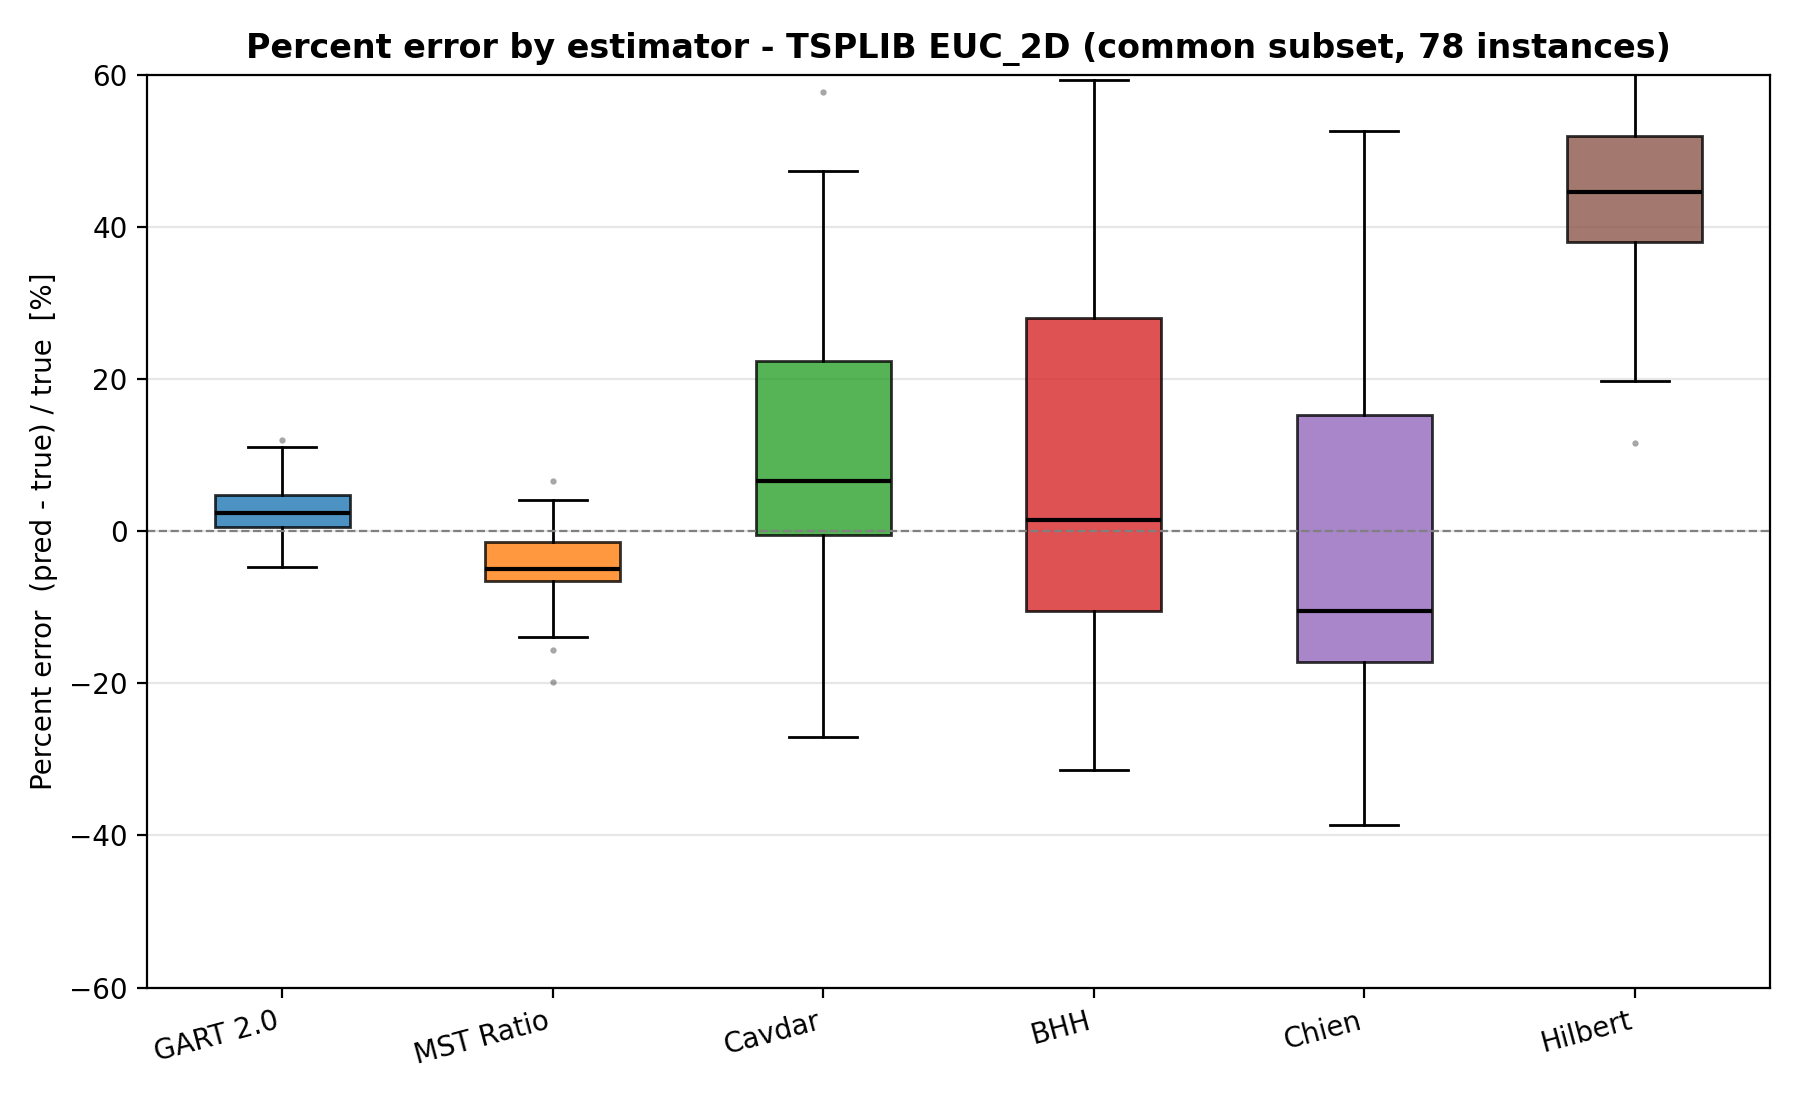
\includegraphics[width=0.75\textwidth]{boxplot_tsplib_errors.png}
\caption{Percent-error distribution per model on the TSPLIB95 EUC\_2D subset (78 instances).}
\label{fig:boxplot_tsplib}
\end{figure}

GART 3.0 transfers from synthetic to real-world with 3.44\% MAPE and 3.52\% SDPE --- tighter than every classical baseline including MST Ratio (5.22\% / 4.54\%). The largest instance ($n = 85{,}900$, 86$\times$ the training cap) is predicted in under 0.5~s. BHH, Cavdar, and Chien all degrade past $n = 500$, where real-world instances violate the uniform-density assumption their derivations require; MST Ratio tracks GART within 2\% at $n \ge 1000$, consistent with the dimensional convergence observed in the ND benchmark.

\subsection{Discussion}

GART 3.0 leads every benchmark on both accuracy and precision. Three patterns explain the result and its boundaries.

\textbf{MST Ratio converges to GART at high density.} At $d = 100$, MST Ratio drops to 6.54\% MAPE while GART reaches 0.90\%; at TSPLIB $n > 5000$ the two differ by under 1\% on MAPE. The gap narrows because $\alpha \to 1$ as dimension or density grows, and any fixed constant near 1 is a decent approximation in that regime \citep{percus1996}. GART's advantage is largest in the low-to-mid density regime where $\alpha$ varies most with instance topology --- exactly the regime that dominates practical logistics.

\textbf{Geometric estimators are inapplicable in $d \ge 3$.} BHH, Cavdar, and Chien all require the convex hull area or bounding box volume. Hull computation costs $O(n^{\lfloor d/2 \rfloor})$ \citep{orourke1998} and the hull-to-box volume ratio shrinks exponentially with $d$ \citep{carlsson2024upper}, so these baselines are absent from the ND results by construction.

\textbf{Cost structure.} TSPLIB logs are the only timing logs in our pipeline that cleanly separate preparation from inference; on that benchmark GART 3.0 spends 74.8\% of wall time in feature extraction and MST construction and 25.0\% in LightGBM inference, versus $\ge 99\%$ feature/MST for classical baselines. GART's overhead relative to a classical baseline is the feature pipeline, not the tree ensemble --- and the pipeline cost is already sunk for any MST-based estimator.

GART's known weak points are grid lattices and near-linear manifolds (Line Noise 10.86\% MAPE in Table~\ref{tab:2d_by_size}) where MST topology becomes structurally degenerate. These cases are rare in real logistics but useful for mapping the model's boundary. Overall the approach is viable across dimensions and distributions, with clear headroom in the regime where exact solvers become expensive.

\section{Application: Non-Euclidean Estimation via MDS Embedding} \label{sec:application}

TSPLIB95 contains 33 instances that are not native EUC\_2D: 4 CEIL\_2D (Euclidean with ceiling-rounded distances), 2 ATT (pseudo-Euclidean), 10 GEO (great-circle geographic), and 17 EXPLICIT (distance-matrix only, including the structural outlier \texttt{brg180}). Classical estimators cannot process these: BHH and Cavdar require 2D coordinates, Chien requires convex hull area, and Hilbert requires a Euclidean embedding. This section presents GART 3.0 on these cases. We report timings as an exploration of capability, not as a comparison.

\subsection{MDS preprocessing}

Classical multidimensional scaling embeds an $n \times n$ distance matrix $D$ into $k$-dimensional Euclidean coordinates by eigendecomposing the doubly-centered squared-distance matrix $B = -\tfrac{1}{2} J D^{(2)} J$ with $J = I - \tfrac{1}{n}\mathbf{1}\mathbf{1}^\top$ \citep{borg2005mds}. The embedding is $X = V_k \Lambda_k^{1/2}$. We pick the smallest $k$ retaining $\ge 99.9\%$ of eigenvalue variance, capped at $k = 100$. GART 3.0's MST features are computed from the \emph{original} distance matrix (preserving metric accuracy), while its geometric features use the embedded coordinates. The selected $k$ is passed to the model as the dimension feature. Appendix~\ref{app:mds} gives the derivation.

\subsection{Results on non-Euclidean TSPLIB95}

\begin{table}[!ht]
\centering
\caption{GART 3.0 on non-Euclidean TSPLIB95 (33 instances + \texttt{brg180}). The embedded dimension $k$ is selected per instance by MDS variance retention.}
\label{tab:tsplib_nonEuc}
\resizebox{\textwidth}{!}{%
\footnotesize
\begin{tabular}{@{}l r r r r r r r@{}}
\toprule
Distance type & $N$ & MAPE (\%) & SDPE (\%) & Median (\%) & $R^2_\alpha$ & Time (ms) & Embed. $k$ (avg, range) \\
\midrule
CEIL\_2D        & 4  & 7.11 & 5.66 & 6.96 & $-0.786$ & 550 & 2 \\
ATT             & 2  & 4.40 & 0.83 & 4.40 & $-1.166$ & 17  & 53 (6--100) \\
GEO             & 10 & 4.44 & 2.61 & 4.95 & 0.810    & 57  & 16 (2--61) \\
EXPLICIT (metric) & 16 & 5.94 & 5.85 & 5.19 & 0.391   & 60  & 38 (8--100) \\
\midrule
\texttt{brg180}$^{\dagger}$ & 1 & 160.0 & --- & 160.0 & --- & 2 & 2 \\
\bottomrule
\multicolumn{8}{l}{\footnotesize $^{\dagger}$ Structural outlier: 90 co-located node pairs and 85{,}368 triangle-inequality violations yield} \\
\multicolumn{8}{l}{\footnotesize true $\alpha = 0.436 < 1$, which metric-TSP MST bounds forbid. Reported separately, excluded from aggregates.}
\end{tabular}%
}
\end{table}

GART 3.0 generalizes across all four non-Euclidean distance types with 4--7\% MAPE. GEO instances achieve the lowest error (4.44\%) because great-circle distances admit a low-stress Euclidean embedding at typical geographic scales. EXPLICIT distances reach 5.94\% because their matrices may mildly violate the triangle inequality, inflating MDS stress. The structural outlier \texttt{brg180} is a bridge graph with $\alpha < 1$: its distance matrix is not a metric in the sense required by the MST lower bound, and no MST-based estimator can recover its true tour length. We report it as a limit case, not a failure mode.

\begin{figure}[!ht]
\centering
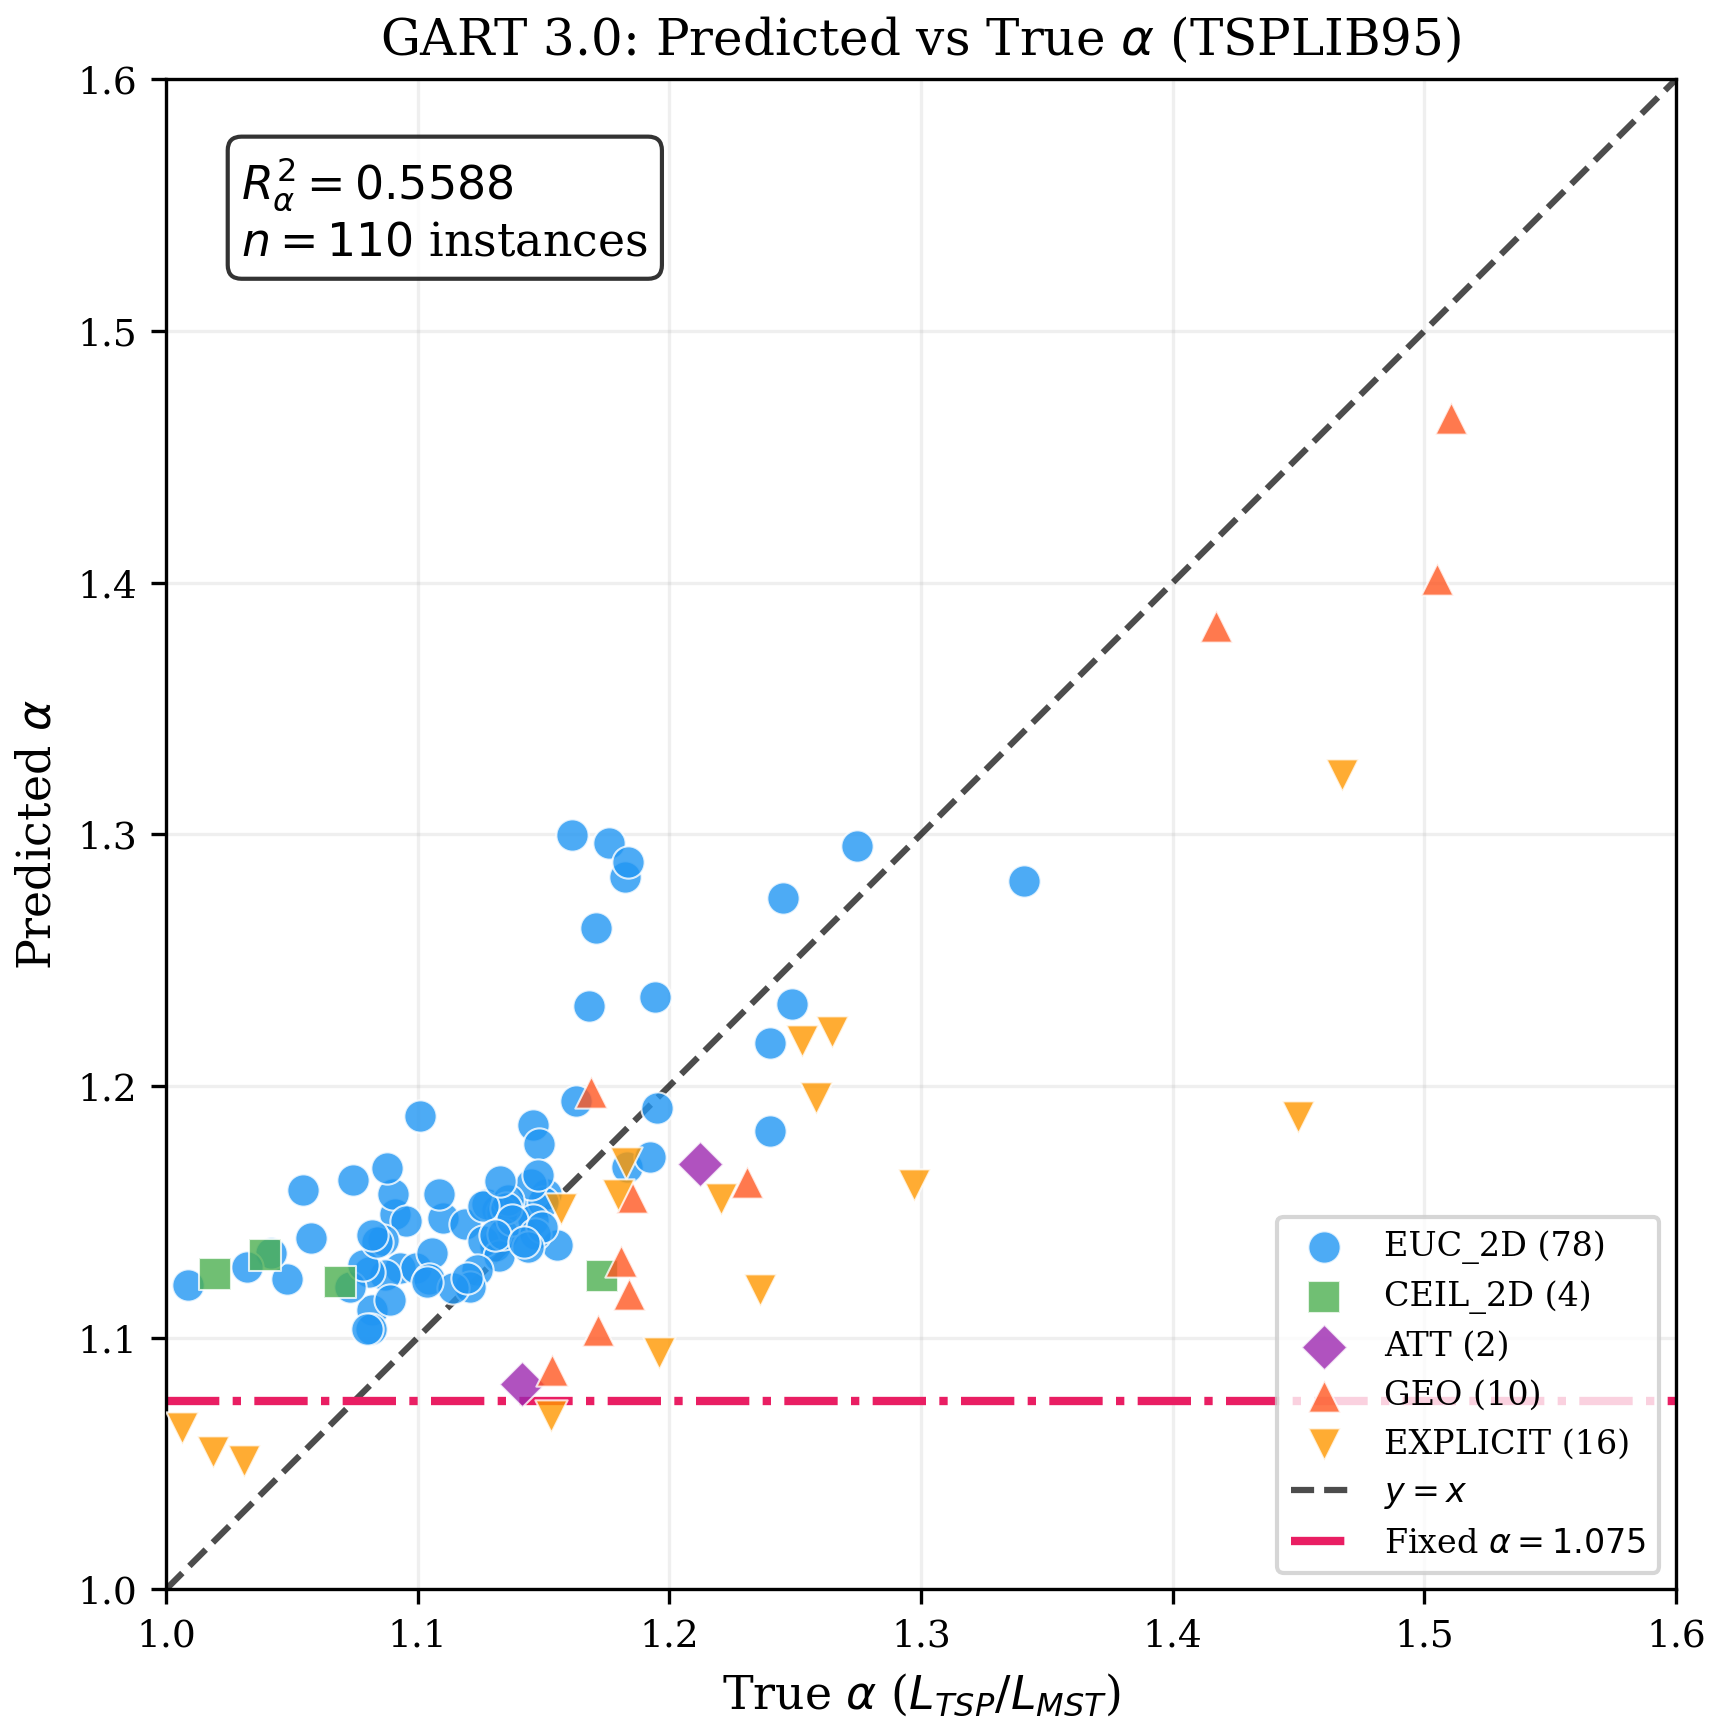
\includegraphics[width=0.75\textwidth]{tsplib_extrapolation.png}
\caption{GART 3.0: predicted vs.\ true $\alpha = L_{\text{TSP}} / L_{\text{MST}}$ on all 111 TSPLIB95 instances, colored by distance type.}
\label{fig:tsplib_scatter}
\end{figure}

Figure~\ref{fig:tsplib_scatter} places all 111 TSPLIB95 instances (78 EUC\_2D from Section~\ref{subsec:results} plus 33 non-Euclidean) on a single predicted-versus-true $\alpha$ plot. Predictions cluster along the diagonal across all five distance types, showing that the MST-to-TSP scaling factor is learnable even when coordinates are derived rather than native. Average inference time across the 33 non-Euclidean instances is 37~ms, dominated by MDS eigendecomposition and MST construction rather than LightGBM evaluation. This enables tour-length estimation for logistics problems defined on road networks, travel times, or other non-Euclidean metric spaces in real time.

